\documentclass[]{article}

\usepackage{mathtools}
\usepackage{listings}
\usepackage{clrscode}
\usepackage{algorithm}
\usepackage{algorithmic}
\usepackage{graphicx}
\usepackage[top=2cm, bottom=2cm, left=2cm, right=2cm]{geometry}
\DeclareMathOperator*{\argmin}{arg\,min}
\DeclareMathOperator*{\argmax}{arg\,max}

\title{Homework 1}
\date{2015-11-16}
\author{Jingwei Zhang 201528013229095}

\begin{document}
    \maketitle
    \section{Problem 1}
    %\begin{figure}[H]
    %    \centering
    %    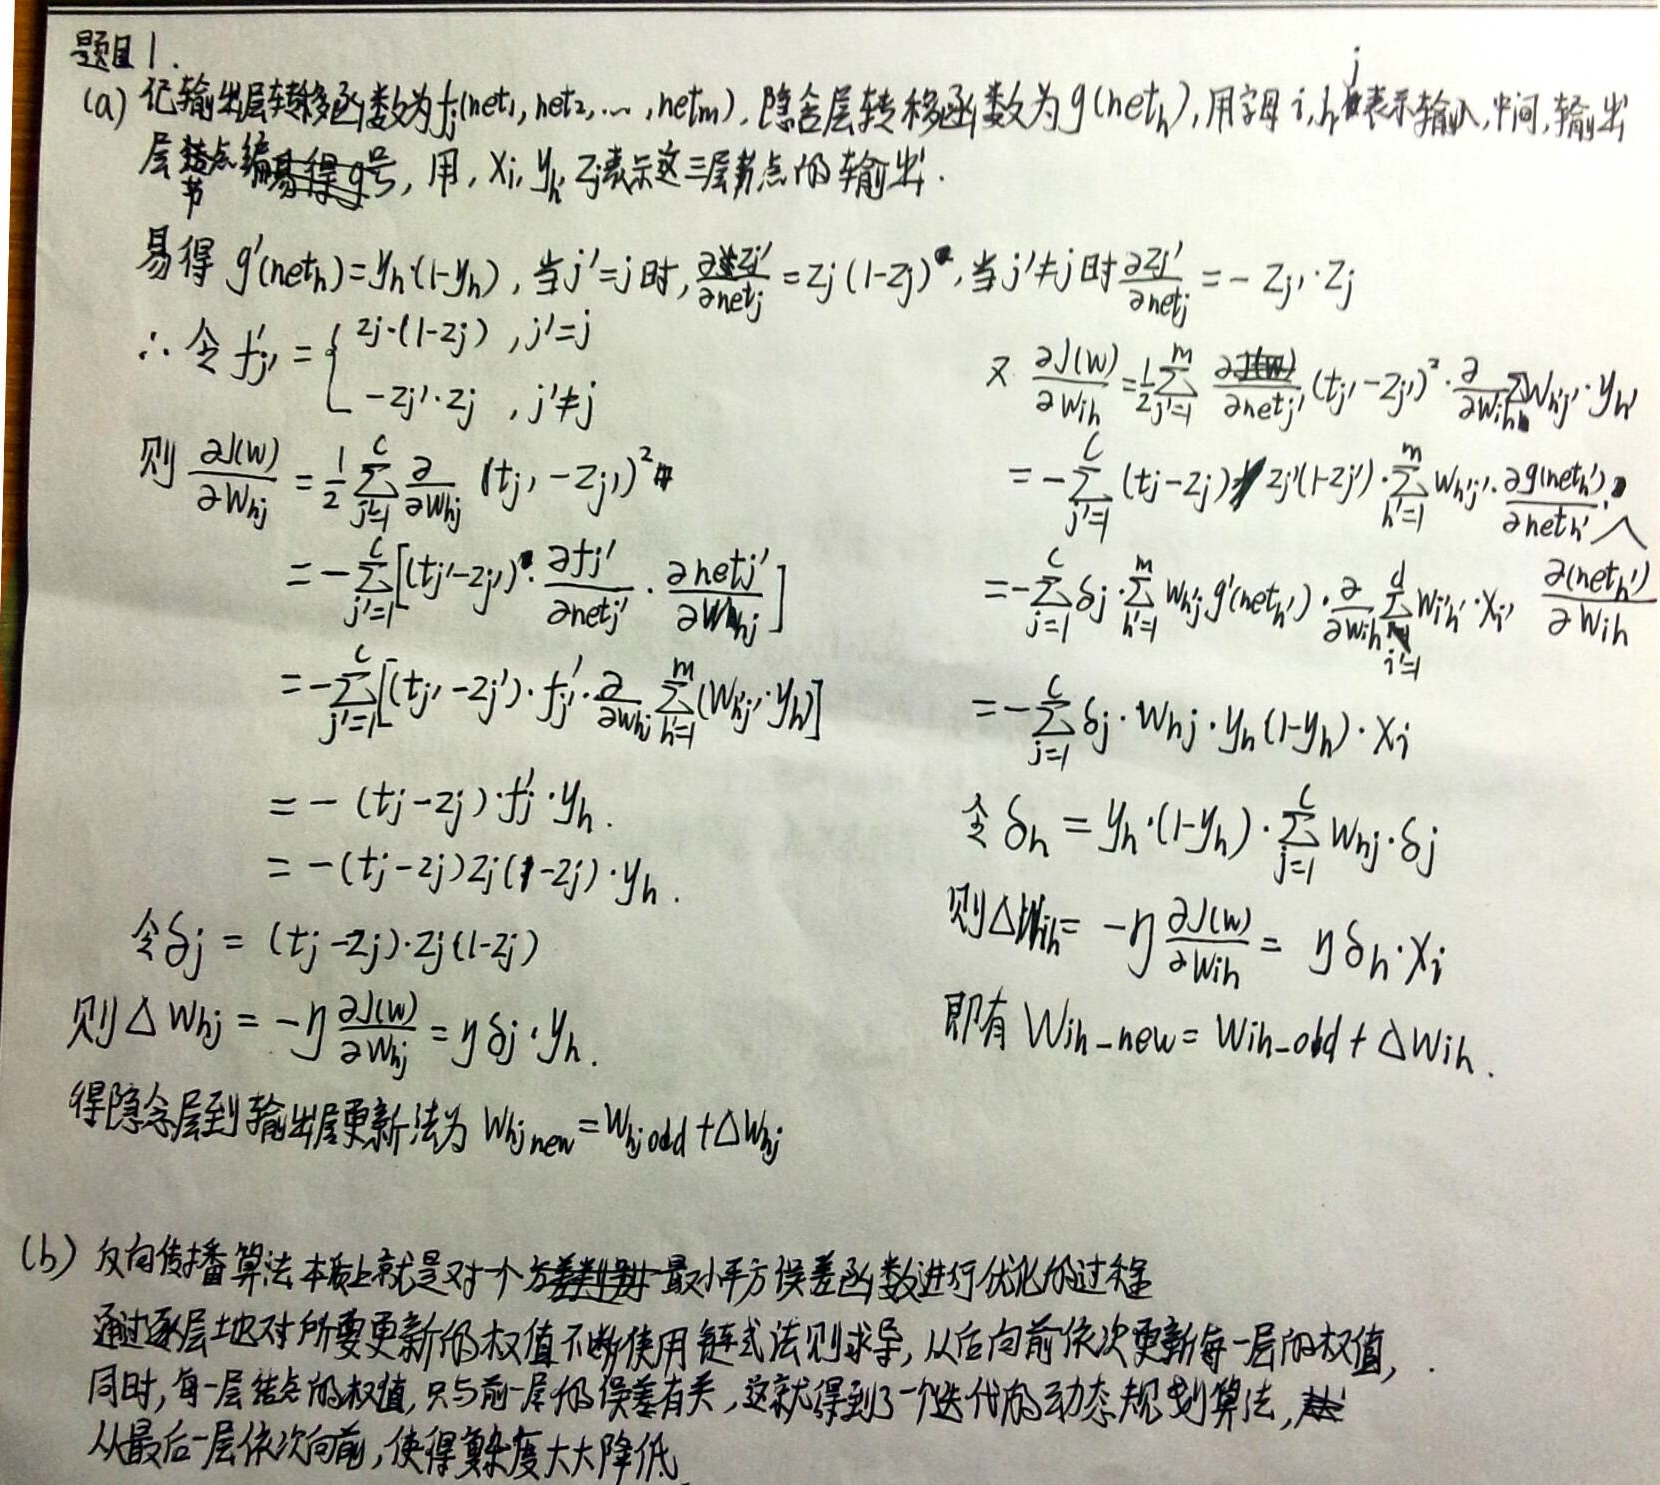
\includegraphics[scale=0.15]{P1.jpg}
    %\end{figure}
    \section{Problem 2}
    \section{Problem 3}
    \section{Problem 4}
    
    \section{Programming Problem 1}
    \subsection{Result}
    
    \subsection{Code}
    \lstinputlisting[language=Python]{1.py}
    \section{Programming Problem 2}
    \subsection{Result}
    \begin{figure}[H]
        \centering
        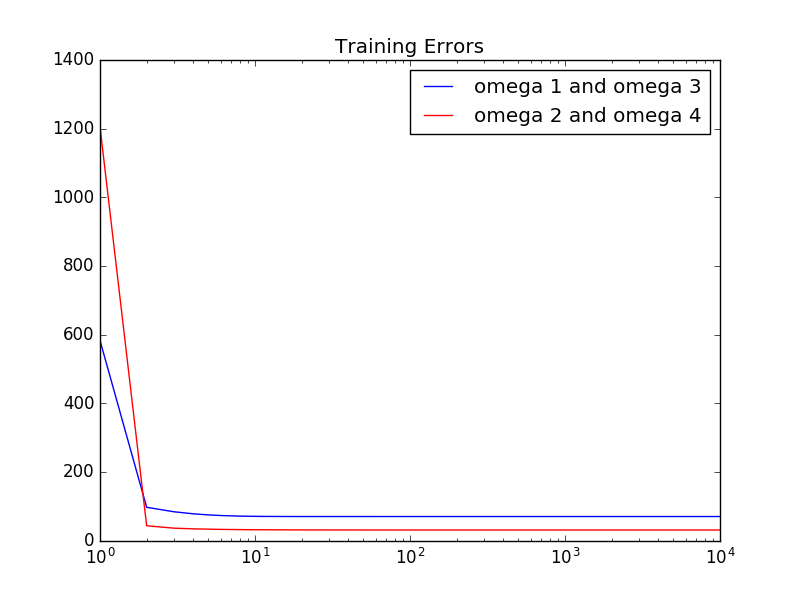
\includegraphics[scale=0.5]{2.png}
    \end{figure}
    \subsection{Code}
    \lstinputlisting[language=Python]{2.py}
    \section{Programming Problem 3}
    \subsection{Result}
    \paragraph{}Batch Relaxation:
    \begin{figure}[H]
        \centering
        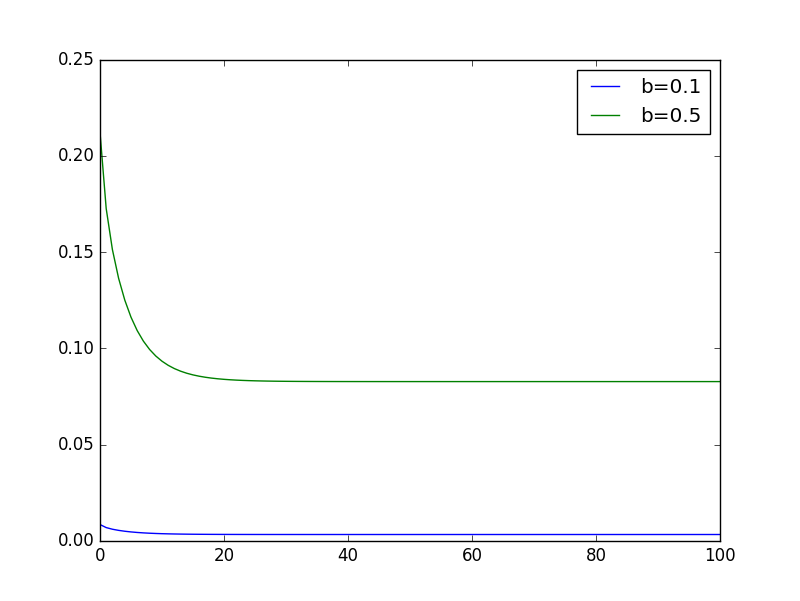
\includegraphics[scale=0.5]{3_batch.png}
    \end{figure}
    \paragraph{}Single Sample Relaxation:
    \begin{figure}[H]
        \centering
        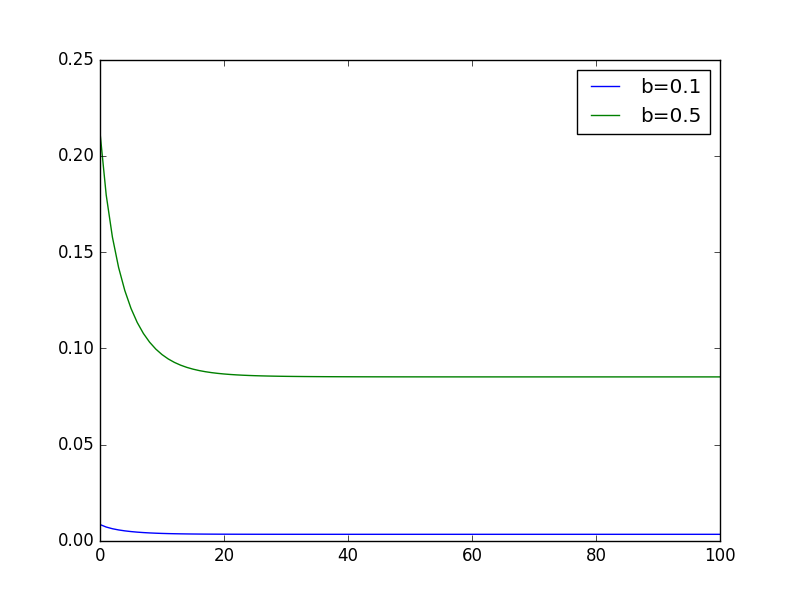
\includegraphics[scale=0.5]{3_single.png}
    \end{figure}
    \subsection{Code}
    \lstinputlisting[language=Python]{3.py}

\end{document}